\documentclass{ctexart}
\usepackage{graphicx} % Required for inserting images
\usepackage{amsmath}
\usepackage{amssymb}
\usepackage{amsthm}
\usepackage{hyperref}
\usepackage{geometry}
\geometry{a4paper, left=1in, right=1in, top=1in, bottom=1in}
\usepackage{minted}
\usepackage{enumitem}

\title{《深度学习基础》第一次实验报告}
\author{PB24000150 李欣宸}
\date{\today}

\begin{document}

\maketitle

本文是我《深度学习基础》的实验报告。实验结果（包含必要的图表）和对实验结果的分析在 \ref{sec:results-and-discussions} 节；实验总结和经验将包含在 \ref{sec:conclusion} 中；代码实现包括 \verb|mlp.py| 和 \verb|load.ipynb|。

\section{实验设置} \label{sec:experimental-setup}

\paragraph{数据集} 本次实验使用的是糖尿病疾病进展数据集（Diabetes dataset），包含442个样本，每个样本有10个医学特征，作为预测目标；训练前我们对输入进行了标准化处理。

\paragraph{模型架构} 参考实验要求，基线模型的架构选择为：2 层隐藏层，每层 16 个神经元，激活函数 ReLU，Adam 优化器，学习率 $10^{-3}$，训练 500 个 epoch；后续的各项对比实验若不声明都将基于此架构进行调整。

\paragraph{训练指标} 后续实验将以 5 折交叉验证（5-fold cross-validation）的平均均方误差（Mean Squared Error, MSE）作为主要评估指标（\textit{最好}的 epoch）；此外，训练损失以及它们在训练过程中的变化也会作为辅助分析的指标。

\section{结果与讨论} \label{sec:results-and-discussions}

\subsection{主要结果}

基线模型（2 层隐藏层，每层 16 个神经元，ReLU，Adam，$lr=10^{-3}$）在 5 折交叉验证上的最优验证误差为 3079.21（MSE），对应第 280 个 epoch。

在测试集上（使用完整训练集训练），该模型的 MSE 为 2753.92，略优于验证误差，这可能是因为没有交叉验证训练数据更为完整，且该模型有不错的泛化能力。

从损失曲线形态看，多个设置都出现了“前期下降较慢，中期快速下降，后期趋缓”的 S 型走势，这一点在学习率较小时尤其明显（\ref{fig:lr-ablation-horizontal}）。一个直接原因是对于 Adam 优化器，其一阶/二阶动量估计需要若干步才能稳定，类似“预热”，等效步长会从偏保守逐步进入有效区间；当动量统计稳定后下降加快，最终在最优点附近因梯度变小而进入平台期。

\subsection{对比实验}

\paragraph{网络深度的影响}

\begin{itemize}[noitemsep]

    \item 该实验固定学习率为 $10^{-2}$，比较 1、2、3 隐藏层（每层 16 单元）；
    \item 三者最优验证误差分别为：1 层 3134.77（第 117 个 epoch），2 层 3110.81（第 46 个 epoch），3 层 3071.66（第 47 个 epoch）；
    \item 深层模型（3 层）达到最优点更快、误差更低，说明在该任务上适度增加深度能提升表示能力；深层模型训练震荡更明显，这与模型结构复杂后损失结构更复杂有关；
    \item 从曲线后段可见，2 层与 3 层的验证误差回升更明显，过拟合风险也更高，可通过早停或正则化缓解。

\end{itemize}

\begin{figure}[htbp]
    \centering
    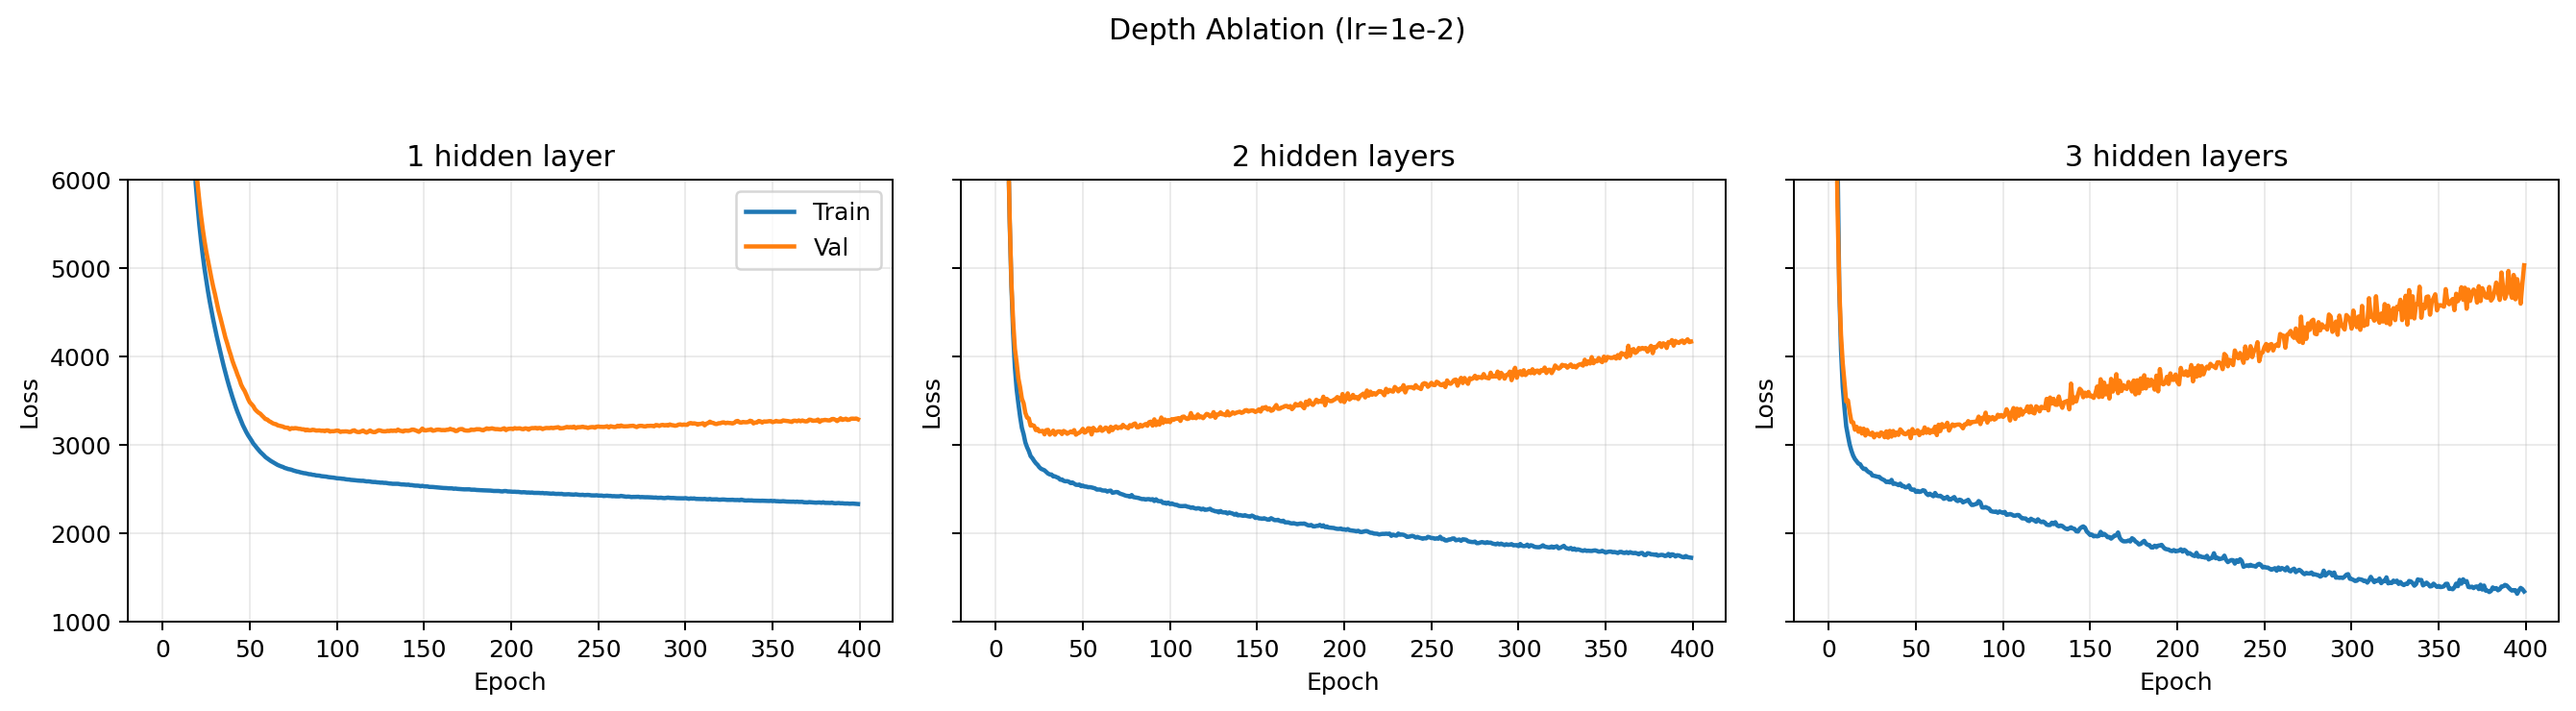
\includegraphics[width=\textwidth]{figures/depth_ablation_horizontal.png}
    \caption{网络深度对比：横向合并训练/验证损失曲线（$lr=10^{-2}$）}
    \label{fig:depth-ablation-horizontal}
\end{figure}

\paragraph{学习率的影响}

我们对比了 $10^{-1}$、$10^{-2}$、$10^{-3}$、$10^{-4}$ 四种学习率，如表 \ref{tab:lr-ablation} 所示：

\begin{table}[htbp]
\centering
\caption{不同学习率的最优验证误差对比}
\label{tab:lr-ablation}
\begin{tabular}{c|c|c}
学习率 & 最优 epoch & 最优验证误差（MSE） \\
\hline
$10^{-1}$ & 21 & 3151.40 \\
$10^{-2}$ & 46 & 3110.81 \\
$10^{-3}$ & 280 & 3079.21 \\
$10^{-4}$ & 3530 & 3061.59 \\
\end{tabular}
\end{table}

实验结果符合预期：学习率越小，其达到最优需要的 epoch 越多，但最终验证误差越低（该实验中我们把 $10^{-4}$ 的训练预算从 500 扩大到 5000 epoch）；不同学习率均有过拟合现象，但学习率越大过拟合速度越快；$10^{-1}$ 时训练出现震荡，但大体稳定，这与 Adam 优化器和该任务较为简单有关。

\begin{figure}[htbp]
    \centering
    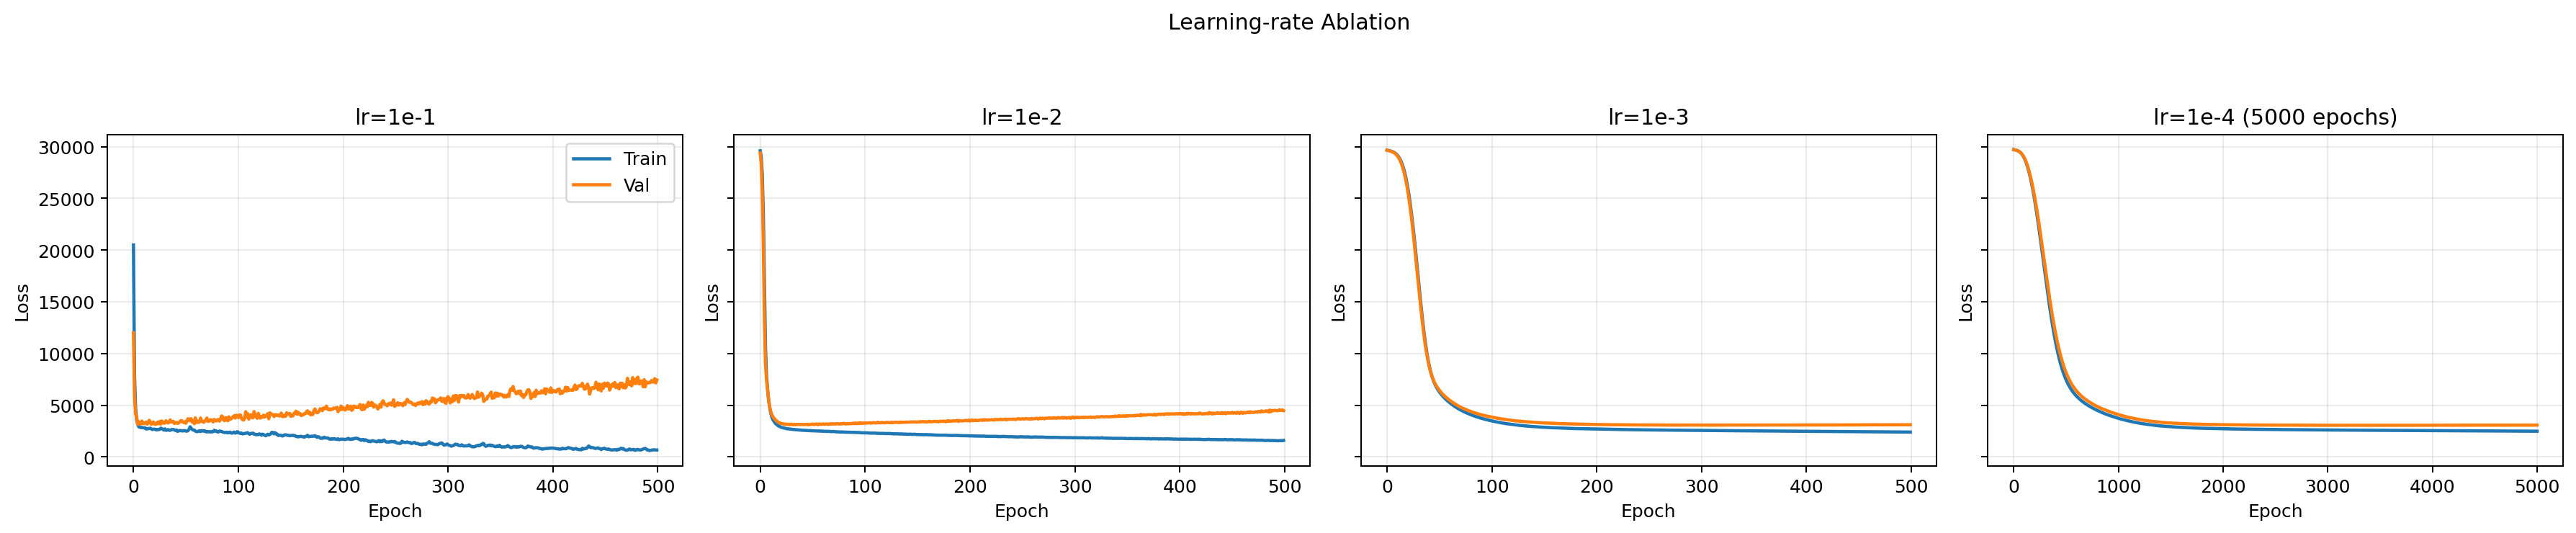
\includegraphics[width=\textwidth]{figures/lr_ablation_horizontal.png}
    \caption{学习率对比：横向合并训练/验证损失曲线（其中 $10^{-4}$ 训练 5000 epoch）}
    \label{fig:lr-ablation-horizontal}
\end{figure}

\paragraph{激活函数的影响}

固定网络为 2 层隐藏层、学习率为 $10^{-2}$，比较 Sigmoid、Tanh、ReLU、LeakyReLU、Swish，如表 \ref{tab:activation-ablation} 所示：

\begin{table}[htbp]
\centering
\caption{不同激活函数的最优验证误差对比}
\label{tab:activation-ablation}
\begin{tabular}{c|c|c}
激活函数 & 最优 epoch & 最优验证误差（MSE） \\
\hline
Sigmoid & 262 & 4089.39 \\
Tanh & 254 & 4026.81 \\
ReLU & 46 & 3110.81 \\
LeakyReLU & 60 & 3099.71 \\
Swish & 27 & 3282.71 \\
\end{tabular}
\end{table}

可以看到，非饱和类激活（ReLU/LeakyReLU）整体优于 Sigmoid/Tanh；LeakyReLU 取得了本组最优结果，说明给负半轴保留小梯度在该小规模回归任务上是有效的。

接下来我们考察 ReLU 的死亡神经元和 Sigmoid/Tanh 的梯度消失问题。我们发现：

\begin{itemize}[noitemsep]
    \item 在该实验中，ReLU 的死亡神经元（即输出恒为 0 的神经元）占比为 $4/32=12.5\%$，且全部出现在第 2 隐藏层；
    \item Sigmoid 和 Tanh 没有对于 $90\%$ 输入数据，输入绝对值都超过 4 的神经元；
    \item 对于单组数据，平均下来 ReLU 有 $67.43\%$ 的神经元处于激活状态（输出非零），而 Sigmoid/Tanh 则有 $43.99\%$ 和 $51.43\%$ 的神经元处于饱和状态（输入绝对值超过 4）；
    \item 我们猜测，Sigmoid 和 Tanh 并没有发生严重的梯度饱和问题，但是由于训练时很多神经元的输入已经进入饱和区，导致它们的梯度较小，训练速度缓慢；ReLU 有死亡神经元但是不明显，可能与模型较浅有关。
\end{itemize}

\begin{figure}[htbp]
    \centering
    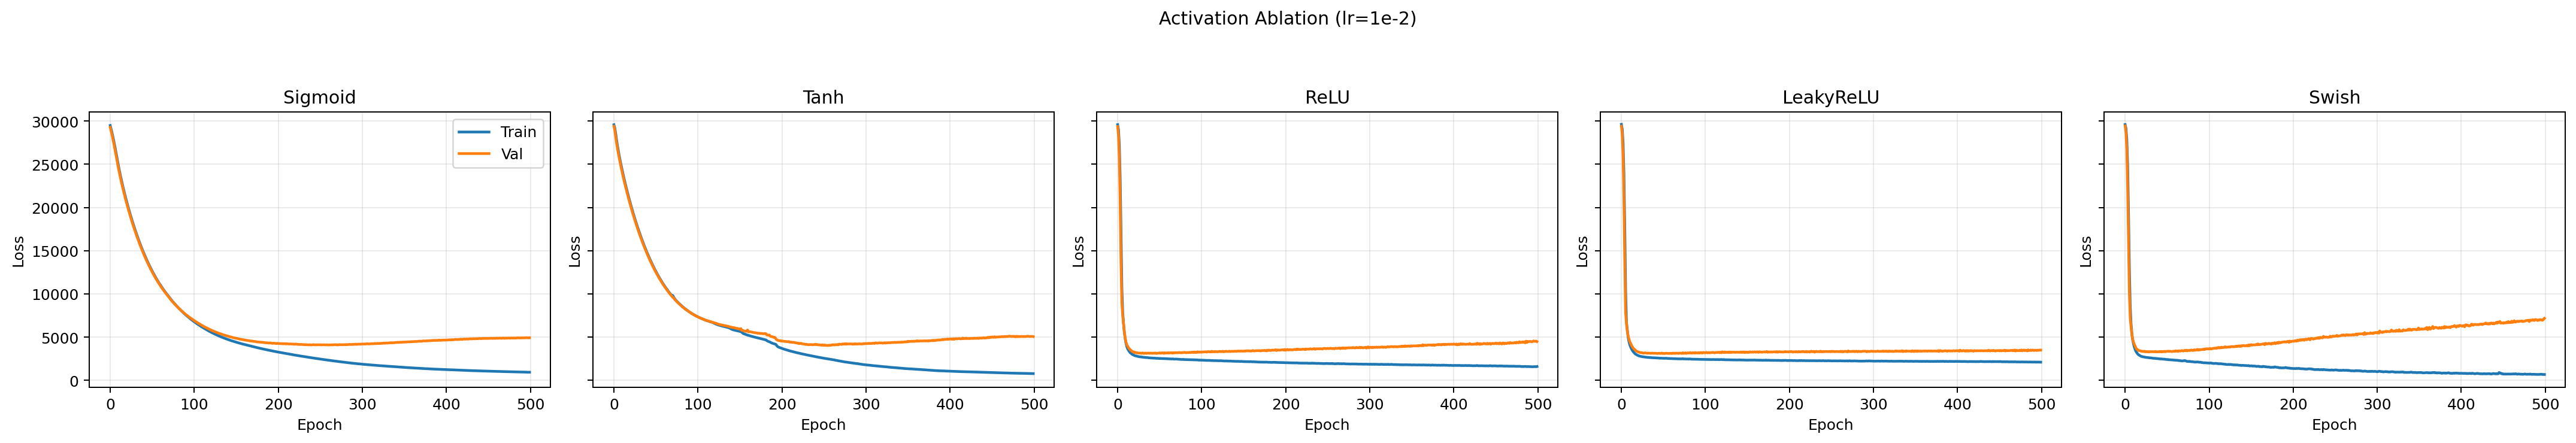
\includegraphics[width=\textwidth]{figures/activation_ablation_horizontal.png}
    \caption{激活函数对比：横向合并训练/验证损失曲线（$lr=10^{-2}$）}
    \label{fig:activation-ablation-horizontal}
\end{figure}

\section{结论} \label{sec:conclusion}

本实验在糖尿病回归任务上完成了 FNN 的实现与三组对比，最终基线模型（2 层隐藏层，每层 16 个神经元，ReLU，Adam，$lr=10^{-3}$）在测试集上取得了 2753.92 的 MSE。对比实验的结论如下：

\begin{itemize}[noitemsep]
    \item 深度方面，3 层隐藏层优于 1 层和 2 层，但过拟合和震荡现象更明显；
    \item 学习率方面，学习率越低；当 $10^{-4}$ 训练到 5000 epoch 时取得全局最优误差（3061.59）；
    \item 激活函数方面，LeakyReLU 表现最好，ReLU 次之，Sigmoid/Tanh 相对落后。
\end{itemize}

\end{document}